\clearpage
\appendix
\section{Archived OULAD control sensitivity}

The archived design and the common-design audit use different adjustment sets. The archived analysis gives an adjusted contrast of $+0.049$ for on-time submission and non-withdrawal. Ordinary pooling shifts the estimate to $+0.075$ (nominal interval $[+0.036,+0.114]$), and signed pooling shifts it to $+0.040$ ($[-0.026,+0.105]$). The common-design results in the main text use the same adjustment set across the target and all six controls.

\begin{center}\small
\begin{tabular}{lrr}
\toprule
Control omitted & Ordinary pool & Signed pool \\
\midrule
Disability & $+0.071$ & $+0.047$\\
Gender & $+0.081$ & $+0.038$\\
Age band & $+0.074$ & $+0.032$\\
Highest education & $+0.079$ & $+0.037$\\
IMD band & $+0.077$ & $+0.034$\\
Previous attempts & $+0.068$ & $+0.050$\\
\bottomrule
\end{tabular}
\end{center}

All six ordinary-pool intervals exclude zero. The signed interval excludes zero only when previous attempts is omitted. Previous attempts records exposure to the module before the current submission and can reflect prior difficulty as well as engagement.

In 10,000 resamples of the six-control panel, the estimated ordinary null mean was $-0.026$ (percentile limits $[-0.044,-0.010]$) and the oriented null mean was $+0.009$ ($[-0.016,+0.036]$). Holding the target estimate fixed while resampling controls gives limits $[+0.013,+0.064]$ for the signed estimate. The fixed-target resampling exercise measures variation from panel composition. The analytical interval also incorporates the estimated target standard error and uses a different spread term.

\clearpage
\section{OULAD sensitivity to hidden confounding}

The E-value for the uncalibrated contrast was 1.31, with an E-value of 1.14 for the confidence limit nearest the null. Under the E-value framework, an unmeasured confounder associated with both submission timing and retention by risk ratios of 1.31 each, conditional on the measured covariates, could move the point estimate to the null. The boundary illustrates other pairs of associations with the same implication.

\begin{center}
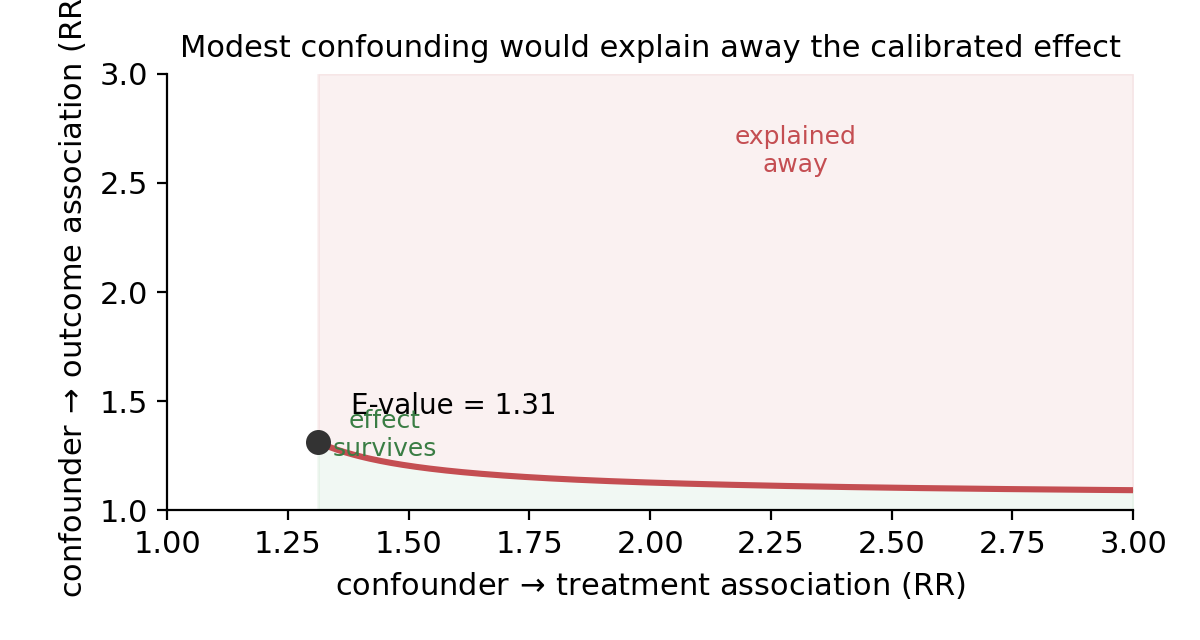
\includegraphics[width=.90\textwidth,height=.52\textheight,keepaspectratio]{../manuscript_updated/figures/figure_07.png}
\end{center}

The archived sensitivity analysis also considered alternative definitions of on-time submission. Estimated contrasts were positive across the reported definitions, while only a subset of the corresponding intervals excluded zero. These comparisons use uncalibrated estimates. Changing the treatment definition alters which students are classified as exposed and can change the adjusted contrast even with the same endpoint and analysis pipeline.

\clearpage
\section{Equal-magnitude sign divergence}

Suppose each control has population bias of magnitude $b>0$ on the target scale, the target bias is $b$, and a fraction $f$ of the controls enters the ordinary pool with the opposite orientation. The ordinary pool estimates $b(1-2f)$, leaving residual target bias $2bf$. Correct sign alignment leaves zero residual bias under these equal-magnitude conditions.

\begin{center}
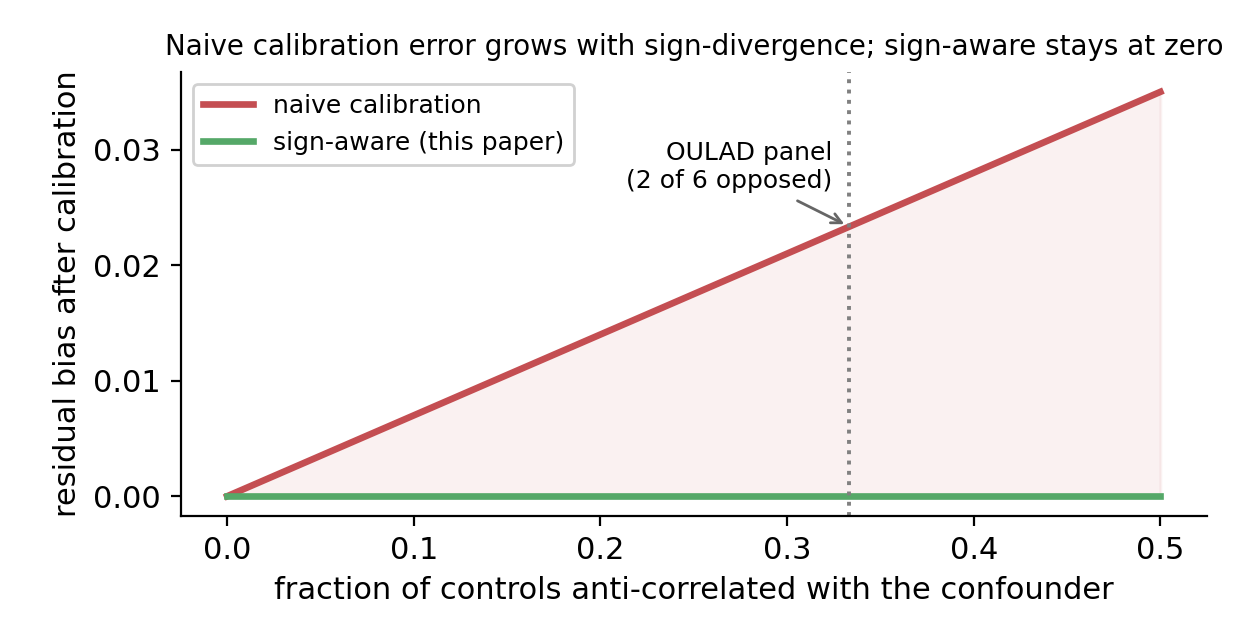
\includegraphics[width=.90\textwidth,height=.50\textheight,keepaspectratio]{../manuscript_updated/figures/figure_08.png}
\end{center}

The figure marks the fraction of flipped signs in the archived OULAD panel for reference. The observed control contrasts are heterogeneous, so that fraction alone cannot determine the sign or magnitude of the empirical correction. More generally, the contribution of an oppositely oriented control to the difference between the two population pools is twice its oriented bias divided by the panel size. One large control can therefore matter more than several weak controls.

\clearpage
\section{Archived known-truth benchmarks}

The original linear benchmark used 1,000 repetitions per setting, 4,000 learners per repetition, six controls and approximately equal bias magnitudes. The table gives the reported residual bias and coverage under ordinary and signed pooling. These results apply to the matched-magnitude benchmark and complement the magnitude and sign perturbations in the main text.

\begin{center}\small
\begin{tabular}{lrrrr}
\toprule
Scenario & Ordinary bias & Signed bias & Ordinary coverage & Signed coverage\\
\midrule
Same signs & $-.001$ & $-.001$ & .94 & .94\\
Opposite fraction $1/6$ & $+.016$ & .000 & 1.00 & .94\\
Opposite fraction $1/3$ & $+.033$ & .000 & .99 & .95\\
Opposite fraction $1/2$ & $+.048$ & $-.001$ & .99 & .94\\
Effect .05, fraction $1/3$ & $+.033$ & .000 & 1.00 & .95\\
\bottomrule
\end{tabular}
\end{center}

\begin{center}
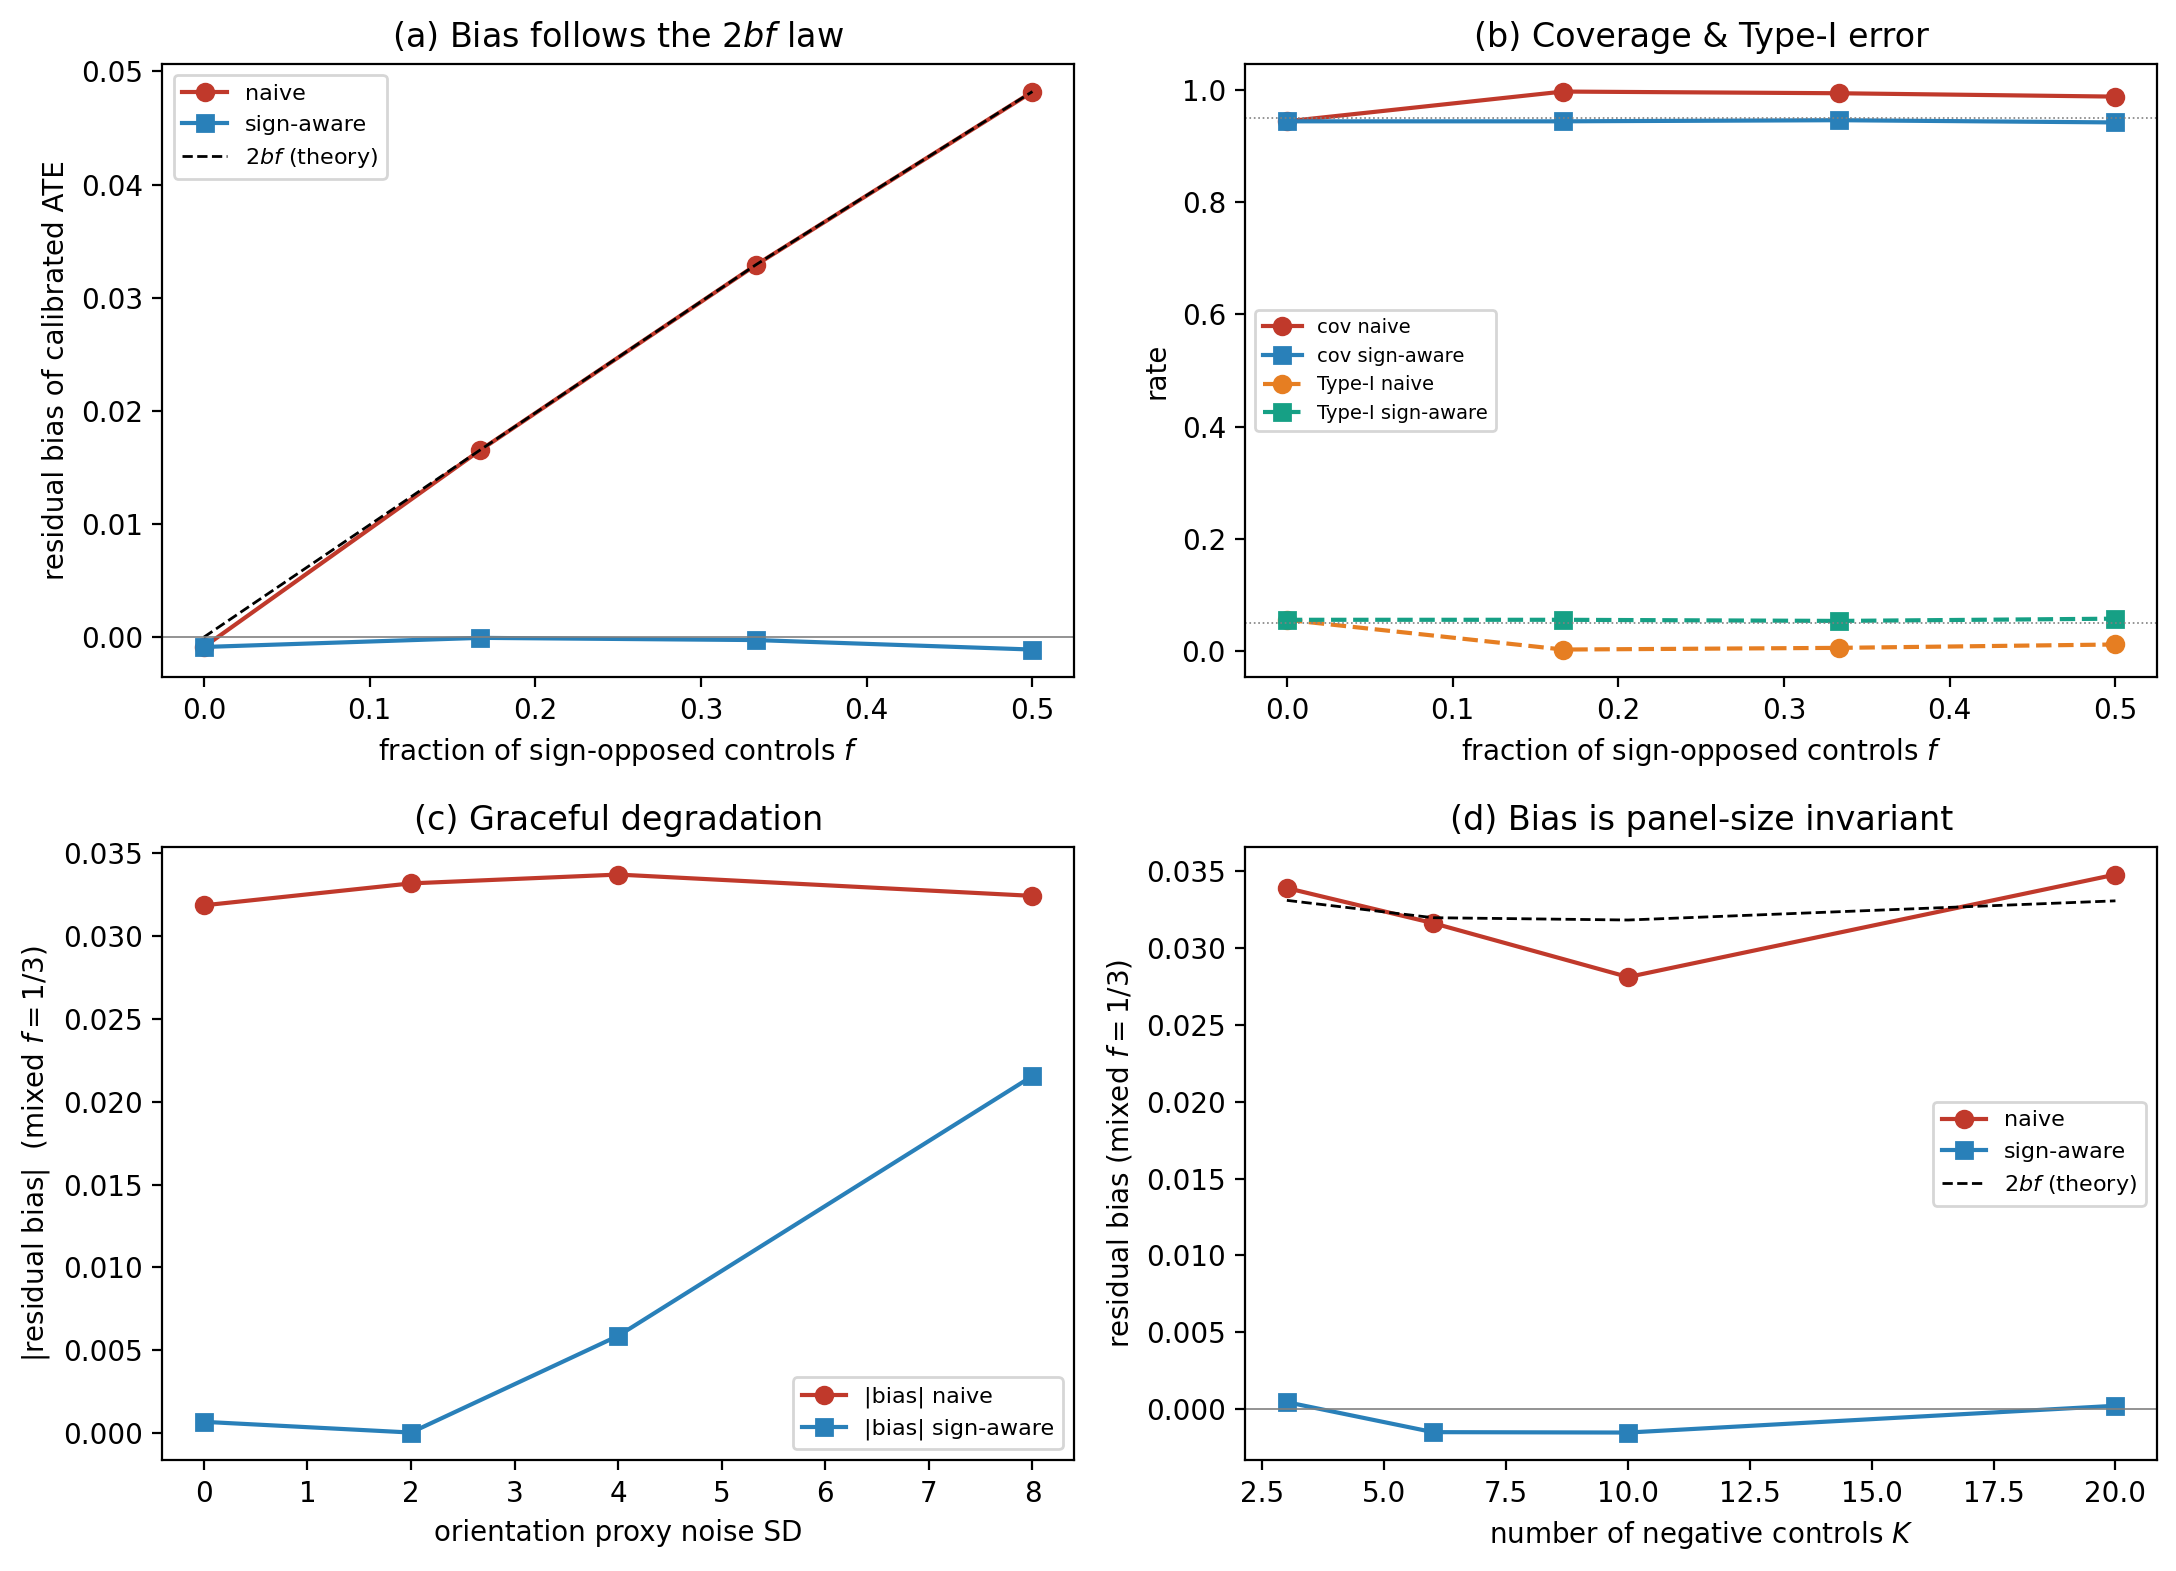
\includegraphics[width=.88\textwidth,height=.38\textheight,keepaspectratio]{../manuscript_updated/figures/figure_09.png}
\end{center}

For the nonzero effect of .05, ordinary pooling rejected zero in 20\% of runs and signed pooling in 66\%. The combination of wide intervals and high coverage illustrates why the binary extension reports mean interval width as well as coverage.

\clearpage
\section{Semi-synthetic OULAD benchmark}

The semi-synthetic benchmark used OULAD covariates and the recorded pre-deadline engagement signal. The simulation assigned treatment through a mechanism driven by engagement and generated an outcome with a known average effect of approximately .123. The fitted nuisance models omitted the engagement variable used for confounding. Six generated control outcomes shared the engagement loading in magnitude, with four entering the pool in the opposite direction.

The raw, ordinary and signed estimates were .231, .270 and .120. We extended this benchmark using standardized pre-deadline log-click engagement $U_1$ and a generated independent standard normal factor $U_2$. Each panel used 500 samples of 2,000 distinct OULAD learners, taking the first registration per learner in module and presentation order. Measured covariates were module, presentation length and registration timing. With $B=.25$ times standardized length minus $.20$ times standardized registration timing, the treatment logit was $.9U_1+.8U_2+B$ and the target logit was $-.3+.85U_1+.65U_2+B+\alpha A$. Truth is the within-sample mean difference in potential outcome probabilities for $\alpha=0,.55$.

Six controls have logits $s_j(\ell_j^\top U+B)$, with two positive and four negative signs. Matched loadings are $(.85,.65)$; proportional loadings multiply this vector by $(.25,.5,.75,1.25,1.5,1.75)$. Mixed loadings are $(.2,.1),(.4,-.4),(.6,.05),(1,-.8),(1.25,.15),(1.5,-1)$. Two-fold logistic AIPW refits all models in each sample using measured covariates and a noisy proxy $U_1+\epsilon$, with $\epsilon$ standard normal. The same proxy determines relative signs. Neither confounder enters the nuisance models directly.

\begin{center}\footnotesize
\begin{tabular}{llrrrrr}\toprule
Panel & Method & ATE & Bias & Coverage & Width & Reject zero \\\midrule
Matched & Raw & 0.000 & +0.143 & 0.000 & 0.091 & 1.000 \\
 & Ordinary & 0.000 & +0.192 & 1.000 & 0.595 & 0.000 \\
 & Signed & 0.000 & -0.002 & 0.964 & 0.099 & 0.036 \\
Matched & Raw & 0.109 & +0.146 & 0.000 & 0.091 & 1.000 \\
 & Ordinary & 0.109 & +0.194 & 1.000 & 0.595 & 0.562 \\
 & Signed & 0.109 & +0.000 & 0.956 & 0.098 & 0.992 \\
Proportional & Raw & 0.000 & +0.143 & 0.000 & 0.091 & 1.000 \\
 & Ordinary & 0.000 & +0.235 & 0.656 & 0.492 & 0.344 \\
 & Signed & 0.000 & +0.010 & 1.000 & 0.260 & 0.000 \\
Proportional & Raw & 0.109 & +0.146 & 0.000 & 0.091 & 1.000 \\
 & Ordinary & 0.109 & +0.238 & 0.602 & 0.492 & 0.998 \\
 & Signed & 0.109 & +0.012 & 1.000 & 0.260 & 0.378 \\
Mixed & Raw & 0.000 & +0.143 & 0.000 & 0.091 & 1.000 \\
 & Ordinary & 0.000 & +0.158 & 0.098 & 0.233 & 0.902 \\
 & Signed & 0.000 & +0.129 & 0.296 & 0.232 & 0.704 \\
Mixed & Raw & 0.109 & +0.146 & 0.000 & 0.091 & 1.000 \\
 & Ordinary & 0.109 & +0.160 & 0.086 & 0.233 & 1.000 \\
 & Signed & 0.109 & +0.131 & 0.314 & 0.232 & 1.000 \\
\bottomrule\end{tabular}
\end{center}
Rejecting zero measures false positives at ATE zero and power otherwise. This benchmark tests the chosen confounding structures on OULAD covariates. Empirical control comparability still requires a substantive argument.


\clearpage
\section{Archived XES3G5M raw-timestamp sensitivity}

The archived raw-timestamp analysis split 6,000 eligible learners at the user level, measured covariates in the first 30\% of interactions and used the middle 30\% to define treatment. Raw regularity was $1/(1+CV)$ of positive successive timestamp intervals. Late accuracy was measured in the final 40\% of interactions. The primary threshold for this archived sensitivity analysis was the development median, .2373.

The support rule excluded 1,986 of 4,800 development learners (41.4\%). For seed 20260626, the uncalibrated estimate was $-.065$ ($[-.142,.012]$)  . The signed estimate was $-.061$ ($[-.138,.016]$). The holdout Qini permutation test gave $p=.947$.

\begin{center}\small
\begin{tabular}{lrr}
\toprule
Development quantile & Signed estimate range & Intervals excluding zero\\
\midrule
.40 & $[-.035,+.031]$ & 0/5\\
.50 & $[-.061,+.007]$ & 0/5\\
.60 & $[+.021,+.070]$ & 1/5\\
\bottomrule
\end{tabular}
\end{center}

The ranges use five fixed user splits (42, 123, 456, 789 and 20260626). Across the resulting 15 analyses the signed contrast ranged from $-.061$ to $+.070$. The raw interval measure and the session-based measure in the main text define distinct exposures. The weak overlap and threshold dependence in the raw-timestamp analysis motivate reporting exposure construction and overlap alongside the calibration results.

\clearpage
\section{Binary-outcome AIPW stress test}
\label{app:binary-stress}

Each cell uses 500 independent samples of 2,000 learners. With independent standard normal variables $U,X,\epsilon,\eta$, treatment is $A=\mathbb{1}\{U+.5X+\epsilon>0\}$ and the measured orientation proxy is $G=U+\eta$. The target outcome has logit $\alpha A+.8U+.4X$. Control $j$ has logit $s_j(l_j U+.4X)$, with alternating $s_j=\pm1$ and no treatment term. The matched loadings are all .8. The weak loadings are $(.15,.20,.25,.30,.35,.40)$ and the dominant panel is $(3.2,.8,.8,.8,.8,.8)$. These are logit coefficients. Residual risk-difference biases also depend on adjustment and the nonlinear link.

The analysis fits logistic propensity and treatment-specific outcome models using $X,G$ in two cross-fitting folds, separately in each replication, and clips estimated propensities to $[.02,.98]$. The true marginal effect is computed by Gaussian quadrature for $\alpha=0$ and $\alpha=.5$. Signs are estimated from the target and control correlations with $G$ in each sample. The signed covariance interval for fixed estimated orientations is available in the replication files.

\begin{center}\small
\begin{tabular}{llrrrrr}\toprule
Panel & Method & ATE & Bias & Coverage & Reject zero & Width \\\midrule
Matched & Uncorrected & 0.000 & +0.121 & 0.006 & 0.994 & 0.104 \\
Matched & Ordinary & 0.000 & +0.120 & 1.000 & 0.000 & 0.528 \\
Matched & Signed & 0.000 & -0.001 & 0.952 & 0.048 & 0.114 \\
Matched & Uncorrected & 0.105 & +0.122 & 0.000 & 1.000 & 0.103 \\
Matched & Ordinary & 0.105 & +0.122 & 1.000 & 0.140 & 0.528 \\
Matched & Signed & 0.105 & +0.001 & 0.954 & 0.960 & 0.114 \\
Weak & Uncorrected & 0.000 & +0.121 & 0.006 & 0.994 & 0.104 \\
Weak & Ordinary & 0.000 & +0.124 & 0.362 & 0.638 & 0.224 \\
Weak & Signed & 0.000 & +0.075 & 0.338 & 0.662 & 0.124 \\
Weak & Uncorrected & 0.105 & +0.122 & 0.000 & 1.000 & 0.103 \\
Weak & Ordinary & 0.105 & +0.126 & 0.360 & 1.000 & 0.224 \\
Weak & Signed & 0.105 & +0.076 & 0.318 & 1.000 & 0.124 \\
Dominant & Uncorrected & 0.000 & +0.121 & 0.006 & 0.994 & 0.104 \\
Dominant & Ordinary & 0.000 & +0.097 & 1.000 & 0.000 & 0.659 \\
Dominant & Signed & 0.000 & -0.024 & 0.996 & 0.004 & 0.243 \\
Dominant & Uncorrected & 0.105 & +0.122 & 0.000 & 1.000 & 0.103 \\
Dominant & Ordinary & 0.105 & +0.098 & 1.000 & 0.000 & 0.659 \\
Dominant & Signed & 0.105 & -0.023 & 1.000 & 0.092 & 0.242 \\
\bottomrule\end{tabular}
\end{center}

